We brought the TLD badges to the medical X-ray collimator set up, where we set the focus to film distance 100 cm. We noted down the badge no and irradiated the badge with x ray keeping the KVp = 100 V and irradiation time 0.1 sec.

\begin{itemize}
    \item FTD = 90 cm
    \item FFD = 100 cm
    \item Field area = $20 \times 20$ cm$^2$
    \item KVp = 100 V
    \item Time = 0.1 sec
\end{itemize}

We then irradiated two badges with 63 mA and 125 mA and tried to find the unknown dose to both TLD badges. While taking the reading in badge reader, the inlet pressure of the gas was adjusted to 2 Kg/cm$^2$.

\subsection{Observation table of Data}

\begin{table}[H]
    \centering
    \caption{Experimental data}
    \begin{tabular}{|c|c|c|c|c|c|c|}
        \hline
        \textbf{Currents} & \textbf{TLD ID} & \textbf{Xray Dose} & \textbf{D1 --} & \textbf{D2 --} & \textbf{D3 --} & \textbf{Avg Dose} \\
        \textbf{(mA)} & & \textbf{(mGy)} & \textbf{Int TL} & \textbf{Int TL} & \textbf{Int TL} & \textbf{(mGy)} \\
        \hline
        & 108 & 0.26 & 421 & 2643 & 2490 & \\
        20 & 153 & 0.26 & 359 & 2653 & 2574 & 0.26 \\
        & 143 & 0.26 & 373 & 2653 & 2477 & \\
        \hline
        40 & 237 & 0.46 & 524 & 4582 & 4661 & 0.46 \\
        \hline
        & 183 & 0.96 & 945 & 9552 & 9715 & \\
        80 & 229 & 0.9 & 937 & 8825 & 9146 & 0.93 \\
        \hline
        & 146 & 1.8 & 1761 & 18495 & 17541 & \\
        160 & 182 & 1.81 & 1703 & 17652 & 18565 & 1.805 \\
        \hline
        & 248 & 2.21 & 2087 & 21607 & 22560 & \\
        200 & 147 & 2.3 & 2127 & 22725 & 23366 & 2.255 \\
        \hline
        & 235 (Background) & 0 & 229 & 479 & 496 & \\
        & 247 (Background) & 0 & 176 & 196 & 259 & 0 \\
        \hline
    \end{tabular}
\end{table}

\begin{figure}[H]
    \centering
    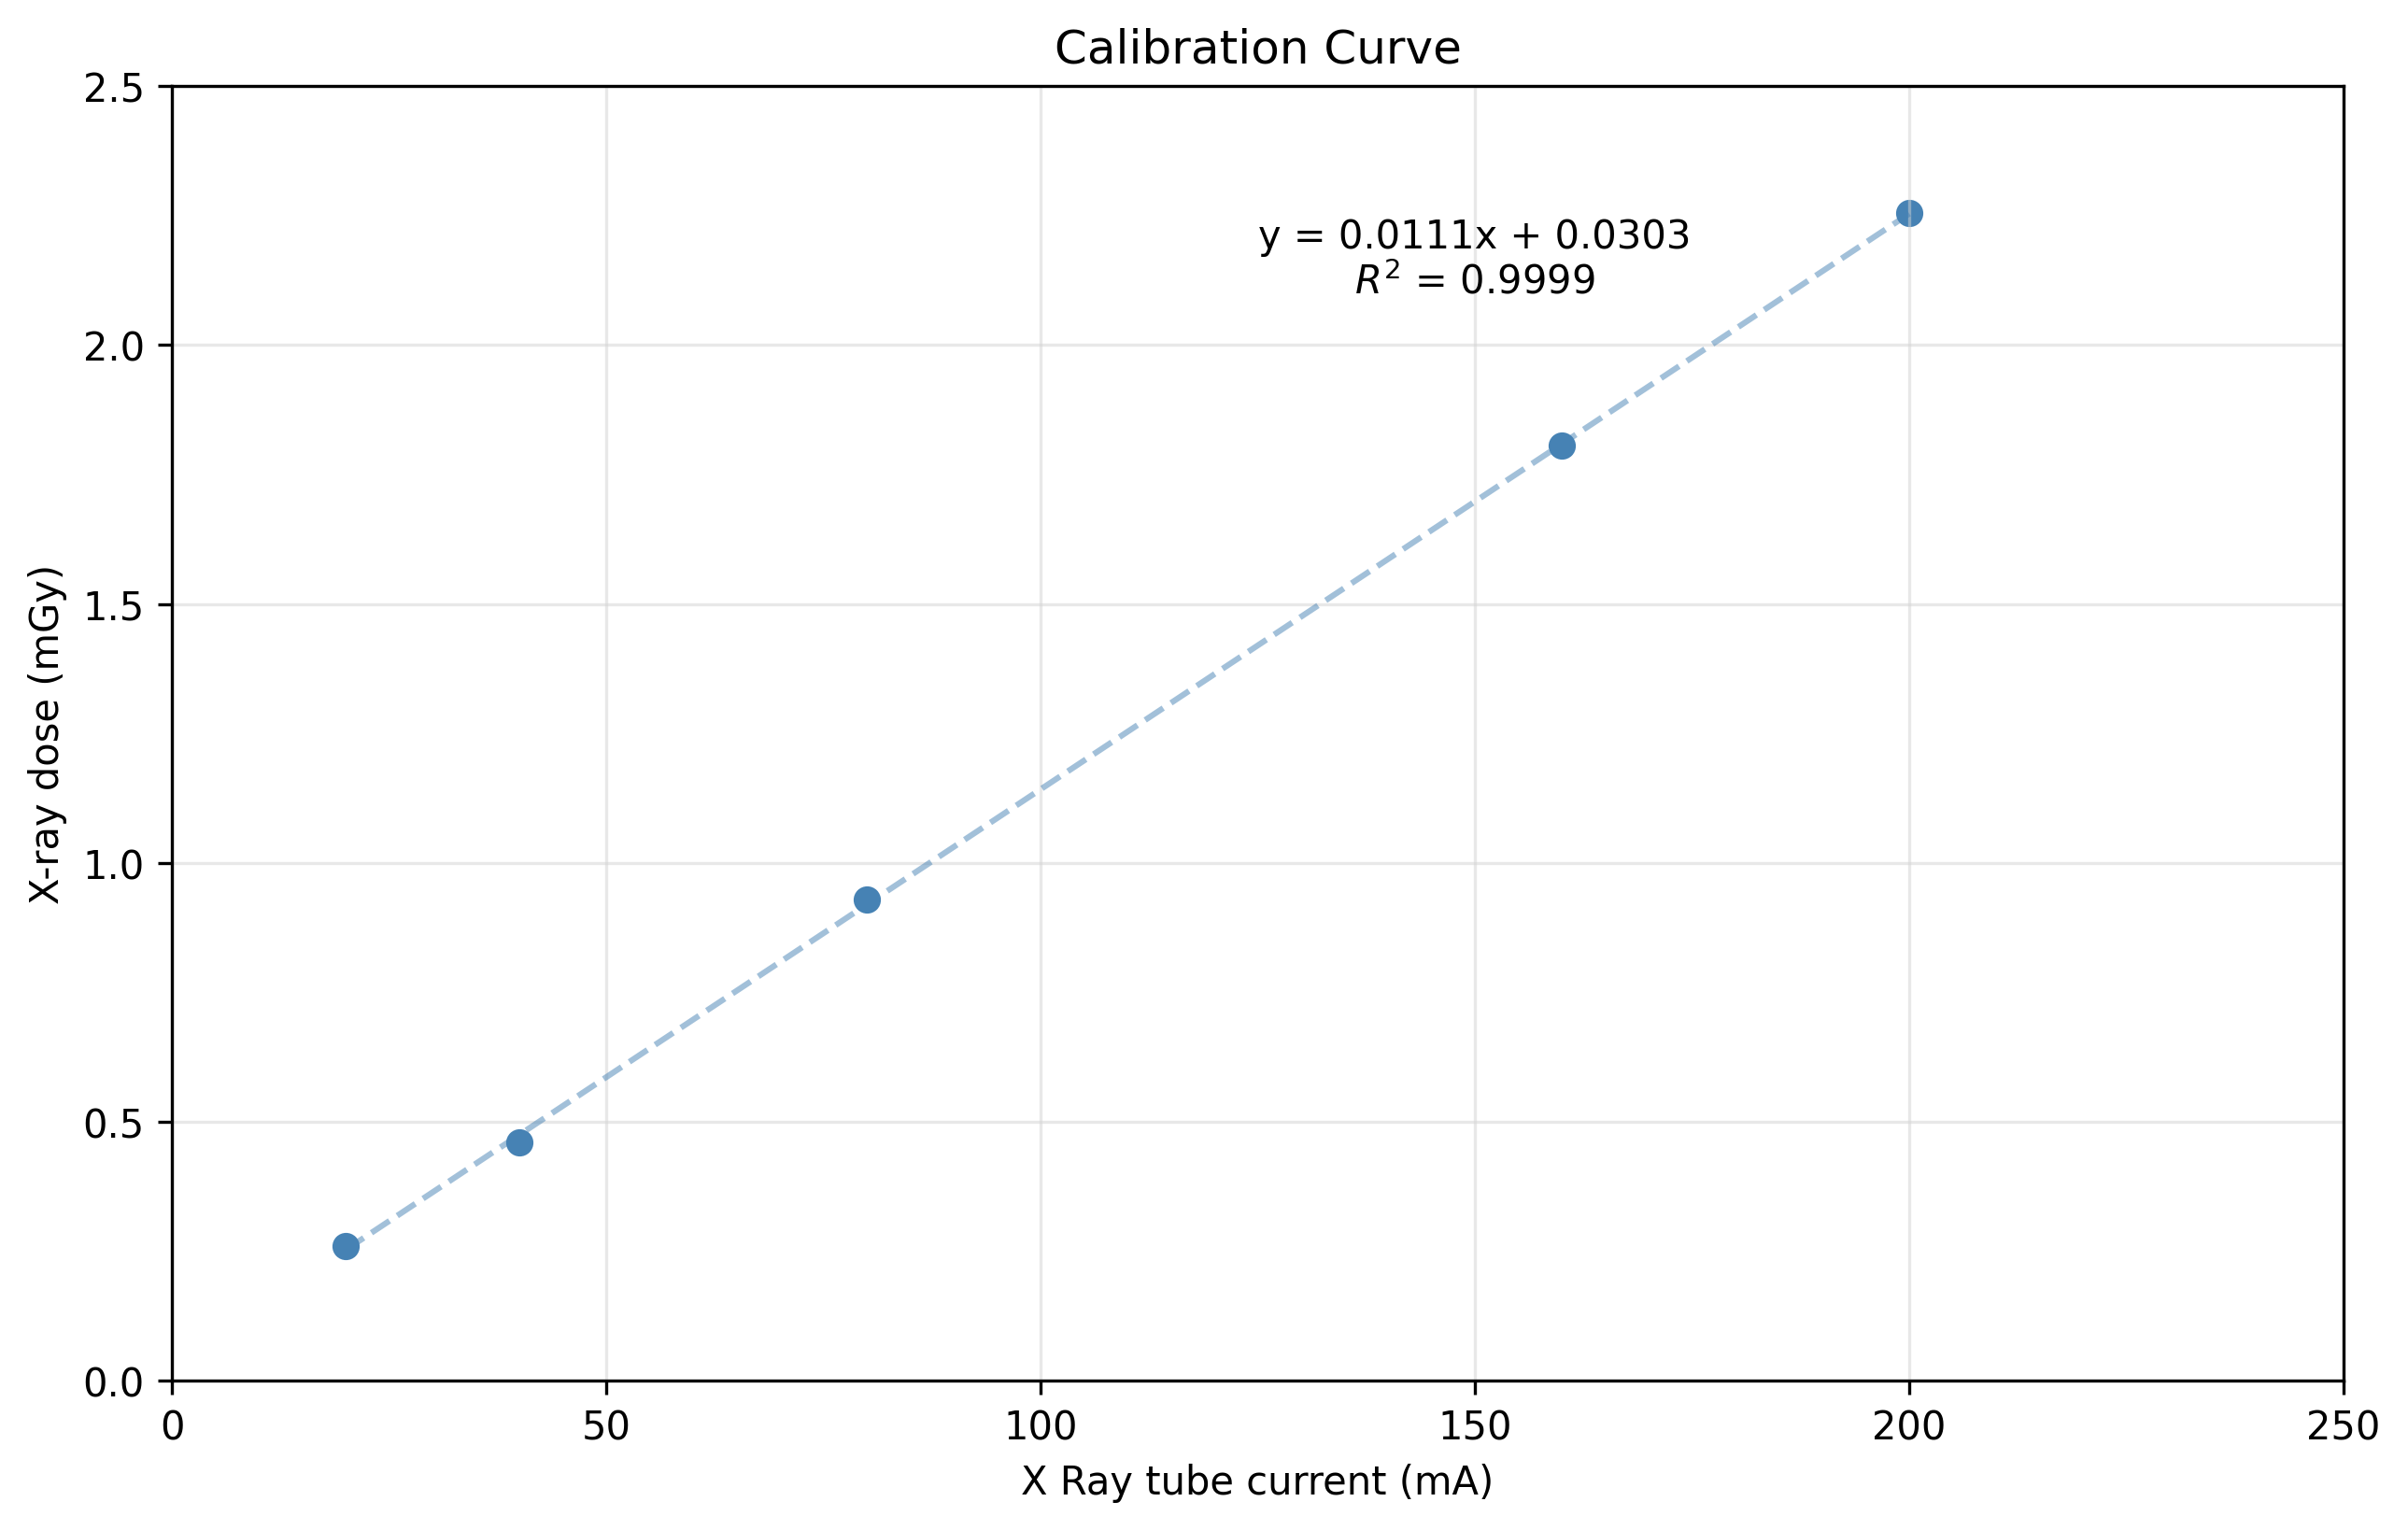
\includegraphics[width=0.8\textwidth]{Figures/calibration_curve.png}
    \caption{Calibration Curve}
\end{figure}

The equation of the curve derived from the experimental plot is:
\begin{equation}
    y = 0.0111x + 0.0303
\end{equation}
This follows the linear form $y = mx + c$, where:
\begin{itemize}
    \item $y$ is the X-ray dose (mGy)
    \item $x$ is the X-ray tube current (mA)
\end{itemize}
So the linearity of the dose with tube current is checked.

\section{Calculation}
Using equation (1), the absorbed dose of TLD card 146 (unknown 1) due to exposure for 63 mA current is given by 0.7296 mGy.

Using equation (1), the absorbed dose of TLD card 108 (unknown 2) due to exposure at 125 mA current is given by 1.4178 mGy.

\subsection{Error Calculation}
According to the TLD badge reader, absorbed dose of TLD 189 (unknown 1) and TLD card 134 (unknown 2) are given by 0.74 mGy and 1.4 mGy respectively. So, the corresponding errors are 1.4\% and 1.2\%.
